	\chapter{Audio}
    	\section{Audio Uses}
        \index{audio}
        \index{audio uses}
          Audio is obviously one of the more important parts of the routine. It can convey significant emotion that the robot by itself cannot. Many times I show people my robot doing a RoboCup performance - but the performance is rather dry in of itself, because the Audio really enhances and provides an explanation to what the robot is doing.\\
        
          The real advantage with the way I constructed the robot's development environment is that I can very accurately animate the robot to the music. This \index{synchronization}\index{sync}synchronization between the robot and the \index{music}music can be used with great effect together.\\
          
          I've also been able to leverage the sync advantage by adding in \index{sound effects}sound effects to the track - such as a roar, and then having the robot roar in sync to the effect. I've also been able to use other effects, such as having the robot sigh, and use "robot motor sounds" to exaggerate it's movement effect.\\
          
          Obviously audio can also be used to tell a \hyperref[Story]{story}, as I'm doing in Nationals. I was inspired by using short snippets of music to tell a \hyperref[Story]{story} by the following \textit{Britain's Got Talent} act:\\
          
          \url{https://www.youtube.com/watch?v=FP7wN301yjc}\\
          
			I didn't want to be restricted to one song - or even one genre in my performances, and that's why I opt to use a mix of songs. Especially at \index{regionals}Regional level people commented that using different genre of music in the performance, in a short period of time really showed off the strengths of the robot - in it's timelessness. Another advantage of using different genres of music is that if one particular song doesn't appeal to some members of the audience, the next genre might.\\
            
            
		\section{Audio Selection}
        	\label{sec:audio_selection}
            \index{audio selection}
        	For every 10 people choosing music for a RoboCup \index{routine}Routine, you'll get 11 different opinions. Because of this I have determined that whilst it's wise to listen to all opinions, ultimately I need to make the decision based upon what I like. Often if I like the selection of \index{audio}audio, in the end, other people do too.\\
            
            On occasions I have selected music or sound effects that didn't particularly compliment the performance, and more than often other people warned me of this. Typically these are small things though, and overall the selection of audio has been complimented. For final decision making, I take other peoples views, consider them, and then make the final decision based upon what I like.\\
            
            I have found that well known music with a beat are typically the favorites. Examples of these are \textit{Gangnam Style - Psy}, \textit{I Feel Good - James Brown}, and \textit{Stayin' Alive - Beegees}. On the other hand, audio such as \textit{Pink Panther Theme}, and \textit{Baby - Justin Bieber} weren't nearly as popular. If it's something you can tap your feet to, it's something that'll work.\\
            
            This is what has caused me the most worry about my \index{nationals}Nationals \index{music}music selection. I've picked a mixture of music that has a good beat, popular, and wel known - but my entire routine is not comprised of it. For example, my opening song for Nationals, \textit{Create/Destroy - Art vs. Science}, is not well known, however has a good beat (and I really like it). \textit{All By Myself - Celion Dion} is well known, but doesn't have as much of a beat. I'm mainly worried because I have none of the songs that have proven their worth previously (Gangnam Style, I Feel Good, Stayin' Alive, etc).\\
            
            This being said, the purpose of this routine isn't to get the audience bobbing their heads - but rather to convey a story, which I feel the selection of music does amply. In short, I'm taking a risk by experimenting - but I think it'll pay off. In the past at Regionals and States my experimentation has typically paid off in my routine being quite unique.\\
            
            \index{final audio selection}
            That being said, here's the final selection of music for Nationals (in order):\\
            
            \begin{enumerate}
            	\item Create/Destroy - Art vs. Science
                \item Clocks - Coldplay
                \item Beat it - Michael Jackson
                \item All by Myself - Celion Dion
                \item Circle of Life - Lion King Theme
            \end{enumerate}
            
		\section{Audio Editing}
        	\index{audio editing}
            \label{audio_editing}
        	If I'm to have multiple songs in the routine, then I need some way to cut them all together. For Regionals and States I used \index{Audacity}Audacity. For Nationals I moved to using \index{Adobe}\index{Adobe Audition}Adobe Audition. Both these are fantastic tools, and a pleasure to learn. Although I'm not particularly skilled in Audio editing, I have did a short course on a camp once, the knowledge of which I was able to employ.\\
            
            \centerline{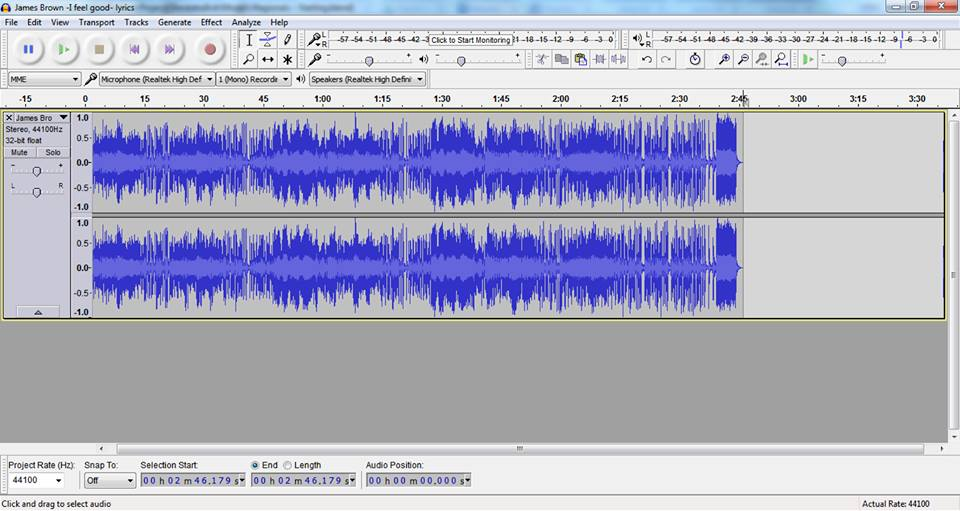
\includegraphics[width=0.75\linewidth]{images/audio_editing}}
            \vspace{10pt}
            
            \centerline{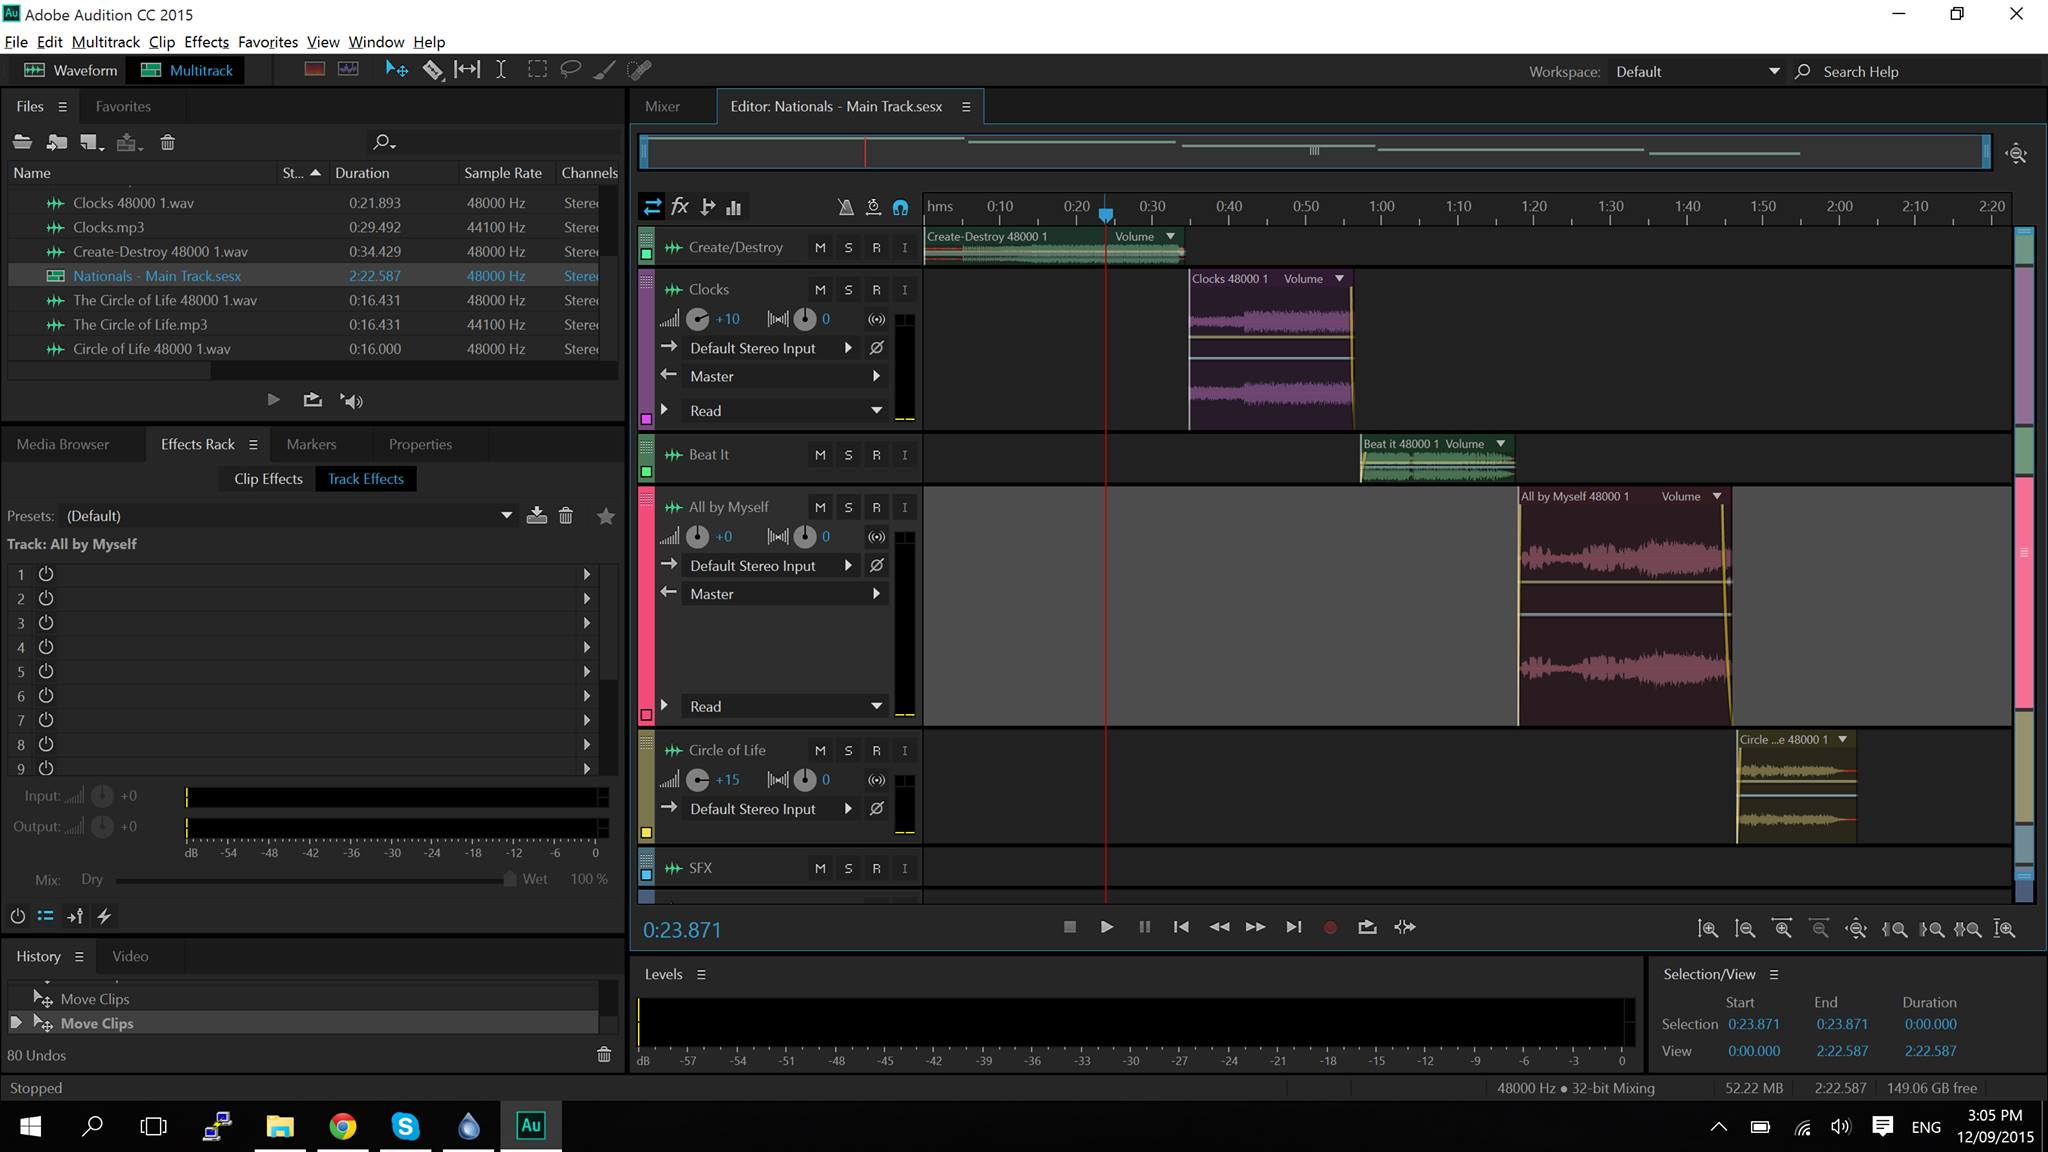
\includegraphics[width=0.75\linewidth]{images/audition_audio_editing}}
            \vspace{10pt}                        
            
            The biggest problem in editing songs together is figuring out when and how to cut a song. Obviously I can't string 5 full length songs together, so I need to cut out the parts I want. Typically I like to keep each individual song to 20-30 seconds each. I try to find a place which I can cut it in that vicinity.\\
            
            I employ two major techniques to gain a cleaner cut if where I'm cutting the song is not clean in of itself:\\
            
            \subsection{Fade In/Fade Out}
            	This one is somewhat self explanatory, fading in and out is a great way to soften unclean cuts.\\
                
			\subsection{Cutting Parts of the Song Together}
            	Sometimes you're able to cut the beginning of a song to the end. The advantage of this is that you get a clean start (as you are using the start of the song), and a clean end (because you are using the actual end of the song). If you are very careful, you are able to get these two cuts and combine them with no noticeable cut.\\
                
                An example of when I used this was in the \textit{I Feel Good} audio. I cut the start of the song, straight to the end - cutting out the middle lyrics and chorus. I cannot distinguish where I have cut the music together - even when I'm looking for it, so the audience doesn't suspect a thing.\\      
                
		                
                
            
            
            
